\documentclass[tikz,border=10pt]{standalone}
\usepackage{amsmath}
\begin{document}
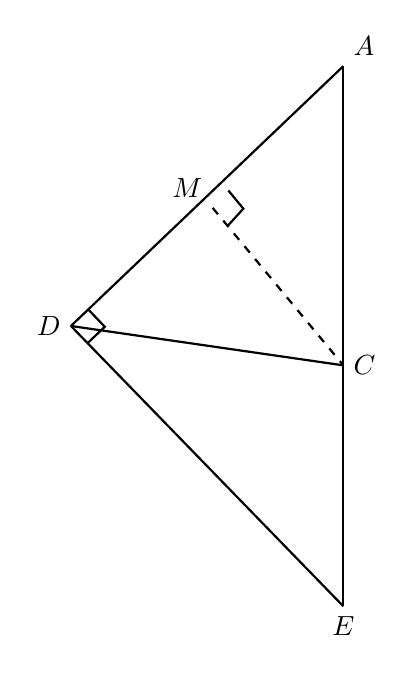
\begin{tikzpicture}[thick, scale=1]
  \coordinate (D) at (1.2,-4.3);
  \coordinate (A) at (4.66,-1.0);
  \coordinate (E) at (4.66,-7.86);
  \coordinate (C) at (4.66,-4.8);
  \coordinate (M) at (3.0,-2.8);

  \draw (D) -- (A);
  \draw (D) -- (E);
  \draw (A) -- (E);
  \draw (D) -- (C);
  \draw[dashed] (M) -- (C);

  % right angle at M
  \draw (3.2,-2.58) -- (3.39,-2.81) -- (3.19,-3.03);
  % right angle at D
  \draw (1.42,-4.09) -- (1.63,-4.31) -- (1.41,-4.52);

  \node[above right] at (A) {$A$};
  \node[above left] at (M) {$M$};
  \node[left] at (D) {$D$};
  \node[right] at (C) {$C$};
  \node[below] at (E) {$E$};
\end{tikzpicture}
\end{document}
